\section{Família Quadrática}

\begin{frame}
\vspace{5pt}
\frametitle{Família Quadrática}
\begin{columns}
\column{0.55\dimexpr\paperwidth-15pt}

Nessa seção, vamos considerar a família de funções $h: [0, 1] \to [0, 1]$ dadas por
$$h(x) = \mu x(1-x),$$
onde $\mu > 1$ é um parâmetro real.
Essa família de funções é conhecia como família quadrática.

\column{0.35\dimexpr\paperwidth-15pt}

\begin{figure}[!htb]
\centering
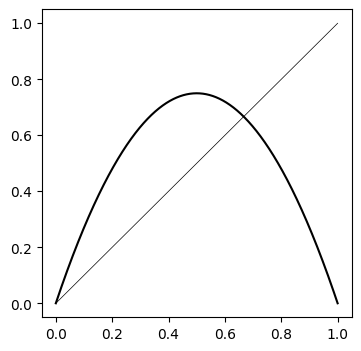
\includegraphics[scale=0.5]{images/h_3.png}
\caption{Gráfico de $h$ para $\mu = 3$.}
\label{h_3,839}
\end{figure}

\end{columns}
\end{frame}

%--------------------
